\chapter*{Benchmarking example 1: Water flow in the soil-root system}

\section*{The model}
\subsection*{The soil sub-problem}
We solve the Richards equation in 3D soil. Since DuMu$^x$ is developed for multi-phase flow in porous media, it uses units of absolute pressure of wetting and non-wetting phases. In the Richards equation, we assume that the non-wetting phase (air) does not change over time and has a constant pressure of 1.0 $\times$ 10$^5$ Pa. Thus, we need to solve only the equation for the wetting phase (water). We stick to the standard DuMu$^x$ units for pressure, although in soil physics, head units are more common, in order to avoid mistakes of e.g. unconsidered hard coded constants, etc. The Richards equation thus can be written as 

\begin{equation}
\frac{\partial}{\partial t} \left(\rho_w \Phi S \right) - \nabla  \cdot \left[\rho_w \frac{\kappa}{\mu}K \left(\nabla p_w-\rho_w \mathbf{g} \right) \right] = \rho_w q_w,
\end{equation}
with $t$ time, $\theta$ water content, $S$ saturation, $\Phi$ porosity, $S \phi = \theta$, $\rho_w$ water density, $K$ intrinsic permeability, $\mu$ dynamic viscosity, $\kappa$ relative permeability, $q_w$ sink term for water uptake, $\mathbf{g}$ gravitational acceleration, $p_w$ absolute pressure of wetting phase (water)\footnote{$p_w$ is the absolute pressure. The matric pressure $p_m$ is defined as $p_m = p_w-p_a$, where $p_a$ is the air pressure, assumed to be constant and equal to 1.0 $\times$ 10$^5$ Pa in this Richards equation model. In order to have head units, we need to convert the water potential from energy per unit volume of water (pressure) to energy per unit weight, i.e., $h_m=\frac{p_m}{\rho_w \mathbf{g}}$}. $\theta$ and $h_m$ are related by the water retention curve: $\theta:= \theta(h)$ (e.g. van Genuchten model)
%and $K_c = \frac{K k_rw \varrho_w g}{\mu_w}$
The simulation domain is a rectangular block of soil, $\Omega_s$, and we prescribe uniform initial conditions and no-flux boundary conditions at the outer faces $\partial \Omega_s$, i.e.,
\begin{eqnarray}
p_w = p_{w,0} & \text{ at } & t=0\\
-\left[\frac{\kappa}{\mu}K \left(\nabla p_w-\rho_w \mathbf{g} \right) \right]\cdot n = 0 & \text{ at } & \partial \Omega_s
\end{eqnarray}

\subsection*{The root system sub-problem}
We solve a modified version of the Richards equation on the branched 1D domain that describes the root architecture. We assume that the root is fully saturated with water, i.e., S=1. We further follow the cohesion-tension theory wherein pressure gradients are the driving force for water movement from soil through plants to the atmosphere. Thus, there is negative absolute pressure inside the xylem\footnote{Water can be liquid at negative pressure (metastable) (Caupin et al. 2013). Constitutive relations e.g. between pressure and density are less known in this state (Davitt et al. 2010). However, in our simulations, we assume constant pressure}.  

\begin{eqnarray}
\overbrace{\frac{\partial}{\partial t} \left(\rho_w \Phi \overbrace{S}^{=1}  \right)}^{=0} - \nabla  \cdot \left[\rho_w K_x\left(\nabla p_w-\rho \mathbf{g} \right) \right] = \rho_w q_{w,r},
\end{eqnarray}
with $K_x$ axial conductance and $q_{w,r}$ the sink term for water uptake by an individual root segment. 

We prescribe zero initial conditions and no-flux boundary conditions at the root tips. At the root collar, we prescribe the water flux equal to the potential transpiration rate T$_{pot}$ as long as the pressure at the root collar is above a certain threshold value. When the pressure at the root collar reaches this threshold value, the boundary condition is switched to a dirichlet condition where the pressure is prescribed to be equal to the threshold value. 
\begin{eqnarray}
p_w = 0 & \text{ at } & t=0\\
-\left[K_x\left(\nabla p_w-\rho \mathbf{g} \right) \right] \cdot n = 0 & \text{ at  the root tips}\\
-\left[K_x\left(\nabla p_w-\rho \mathbf{g} \right) \right] \cdot n = T_{pot} & \text{ at the root collar} & \text { if } p_w > p_{w,c}\\
p_w = p_{w,c} & \text{ at the root collar} & \text{ if } p_w \le p_{w,c},
\end{eqnarray}
where $T{pot}$ is the potential transpiration rate, and $p_{w,c}$ is the critical water pressure (as absolute pressure, permanent wilting point PLUS air pressure!). 

\subsection*{Coupling the soil and root system subproblems}
The soil and root system subproblems are coupled via the sink term for root water uptake. Water flow across the root membrane is driven by the pressure gradient between each root segment and its surrounding soil. 

For each root segment, the radial flux of water $q_{w,r}$ is given by 
\begin{eqnarray}
q_{w,r} = \frac{2 \pi r l K_r}{V_r} (p_{w,root}-p_{w,soil}),
\end{eqnarray}
where $K_r$ is the root hydraulic conductivity, $r$ is the root radius, $l$ is the length of the root segment, $p_{w,root}$ is the absolute pressure inside the root segment, and $p_{w,soil}$ is the local absolute water pressure of the soil at this root segment. 
\todo[inline]{Todo: check where this division by volume is done in the code}

Uptake from soil is computed by summing over the root segments that lie inside each soil control volume $V_s$, i.e.,
\begin{eqnarray}
q_{w,V_s} = \sum_{i=1}^{N}\left(\frac{1}{V_s}(2 \pi r_i f l_i K_{r,i} (p_{w,root,i}-p_{w,soil})) \right),
\end{eqnarray}
where $N$ is the number of root segments that lie inside $V_s$, $f$ is the fraction of root segment length that lies inside $V_s$. 

\section*{The DuMu$^x$ code}
In this chapter, we explain where the different terms of the model equations can be found in the DuMu$^x$ code, i.e., the storage, flux and sink terms. 

\subsection*{The soil subproblem}
The storage and flux terms are defined in the file \\
\verb+/dumux/dumux/porousmediumflow/Richards/localresidual.hh+.\\
The storage term is computed as
\lstinputlisting[firstline=78,lastline=98, language=C++, caption=storage term]{dumux/dumux/porousmediumflow/Richards/implicit/localresidual.hh}		

In the same file, the flux term is computed as 	
\lstinputlisting[firstline=112,lastline=167, language=C++, caption=flux term a]{dumux/dumux/porousmediumflow/Richards/implicit/localresidual.hh}												

The file \verb+fluxvariables.hh+ in the same folder defines the volume flux variable for the Richards equation by setting the nonwetting phase flux variable to zero. 
\lstinputlisting[firstline=50,lastline=70, language=C++, caption=flux term b]{dumux/dumux/porousmediumflow/Richards/implicit/fluxvariables.hh}	

The  definition for the wetting phase (water) is given in\\
\verb+dumux/dumux/porousmediumflow/implicit/darcyfluxvariables.hh+. \\
\lstinputlisting[firstline=19,lastline=349, language=C++, caption=flux term c]{dumux/dumux/porousmediumflow/implicit/darcyfluxvariables.hh}	

The Van Genuchten relationships between saturation and capillary pressure and relative permeability, respectively, are given in \\
\verb+dumux/material/fluidmatrixinteractions/2p/regularizedvangenuchten.hh+.\\

The sink term is defined in the file\\ 
\verb+dumux-rosi/rosi_examples/richardsrootsystem/richardstestproblem.hh+.\\
\lstinputlisting[firstline=245,lastline=265, language=C++, caption=sink term]{dumux-rosi/rosi_examples/richardsrootsystem/richardstestproblem.hh}	

In this file, also the initial and boundary conditions are implemented.
\lstinputlisting[firstline=346,lastline=353, language=C++, caption=initial conditions]{dumux-rosi/rosi_examples/richardsrootsystem/richardstestproblem.hh}	
and
\lstinputlisting[firstline=280,lastline=291, language=C++, caption=initial conditions]{dumux-rosi/rosi_examples/richardsrootsystem/richardstestproblem.hh}	


\subsection*{The root system subproblem}

The description of the source and flux terms can be found in \\
\verb+dumux/dumux/porousmediumflow/1p/implicit/localresidual.hh+
The storage term: 
\lstinputlisting[firstline=79,lastline=91, language=C++, caption=storage term]{dumux/dumux/porousmediumflow/1p/implicit/localresidual.hh}	

The flux term is defined in the same file:
\lstinputlisting[firstline=103,lastline=147, language=C++, caption=flux term]{dumux/dumux/porousmediumflow/1p/implicit/localresidual.hh}	

The corresponding flux variables are defined in \\
\verb+dumux-multidimension/dumux/porousmediumflow/1d/rootsystem/fluxvariables.hh+\\

Inside the root system, water flow is driven by gradients of total pressure, i.e., absolute pressure of water plus gravitational potential. Gravity has only recently been included in the code, the related changes are implemented in the file fluxvariables.hh :
\lstinputlisting[firstline=249,lastline=267, language=C++, caption=gravity]{dumux-multidimension/dumux/porousmediumflow/1d/rootsystem/fluxvariables.hh}	

The sink term is defined in the file\\
\verb+dumux-rosi/rosi_examples/richardsrootsystem/rootsystemtestproblem.hh+.\\
\lstinputlisting[firstline=320,lastline=339, language=C++, caption=sink term]{dumux-rosi/rosi_examples/richardsrootsystem/rootsystemtestproblem.hh}	

In this file, also the boundary conditions are implemented.
Currently, there is a method “Neumann” in which the flux trough the tips is equal to zero and the flux at the collar is prescribed to be the transpirative flux. 
\lstinputlisting[firstline=180,lastline=221, language=C++, caption=sink term]{dumux-rosi/rosi_examples/richardsrootsystem/rootsystemtestproblem.hh}	

\todo[inline]{Todo: Check where in the code we can see the summation over all segments in one soil control volume.}

\subsection*{The input files}
% 
\begin{table}[h!]
	\captionsetup{labelformat=empty}
  \caption{Model input parameters}
  \label{tab:inputs}
  \begin{tabular}{l|c||r}
    \textbf{Parameter}  & \textbf{Units} & \textbf{File number}\\
    \hline
    Water density & kg m$^{-3}$ & 5\\
    Dynamic viscosity & kg s$^{-1}$ m$^{-1}$& 5\\		
    Soil porosity & m$^3$ m$^{-3}$ & 2\\		
		Intrinsic soil permeability & m$^2$ & 1\\
		Residual saturation & - & 2\\	
		Van Genuchten $\alpha$ & Pa$^{-1}$ & 2\\
		Van Genuchten $n$ & - & 2\\		
    Root porosity & m$^3$ m$^{-3}$ & 3\\	
		Root axial conductance & m$^5$ s kg$^{-1}$ & 1\\
		Root radial conductivity & m$^2$ s kg$^{-1}$ & 1\\		
  \end{tabular}
\end{table}

In this subsection, we summarize the required model parameters. All parameter units are based on on absolute pressure and DuMu$^x$ standard units (SI). For comparison with R-SWMS or presentations we convert to “soil physics” standards (matrix potential,…) by pre- and post processing. Currently, required model parameters are distributed across several files:
\begin{enumerate}
   \item \verb+dumux-rosi/rosi_examples/richardsrootsystem/test_rosi.input+.\\
	 \item \verb+dumux-rosi/rosi_examples/richardsrootsystem/richardstestspatialparams.hh+.\\
	 \item \verb+dumux-rosi/rosi_examples/richardsrootsystem/rootsystemtestspatialparams.hh+.\\	
	 \item \verb+dumux-rosi/rosi_examples/richardsrootsystem/grid/Anagallis_femina_Leitner_2010.dgf+.\\		
	 \item \verb+dumux/dumux/material/components/simpleh2o.hh+
\end{enumerate}


Here is the listing of the .input-file: 
\lstinputlisting[language={}, caption=input file]{dumux-rosi/rosi_examples/richardsrootsystem/test_rosi.input}	

\subsection*{Technical issues}
\subsubsection*{Solver}
The default solver of all dumux-rosi examples is an iterative solver. 
In \verb+rositestproblem.hh+ the solver can be set in line 67: 
\begin{lstlisting}
SET_TYPE_PROP(RosiTestProblem, LinearSolver, ILU0BiCGSTABBackend<TypeTag>);
\end{lstlisting}

\subsubsection*{Misc}
Attention: dumux-multidimension master branch currently has a bug (23.02.2017). Switch to another branch: fix/1d-fvelementgeometry

\chapter*{Results}
The results include vtk output for both the soil and the root system domains and can be found in the folder\\
\verb+dumux-rosi/build-cmake/rosi_examples/richardsrootsystem+.\\
The may be visualised using Paraview. 

\begin{figure}[ht]
	\centering
  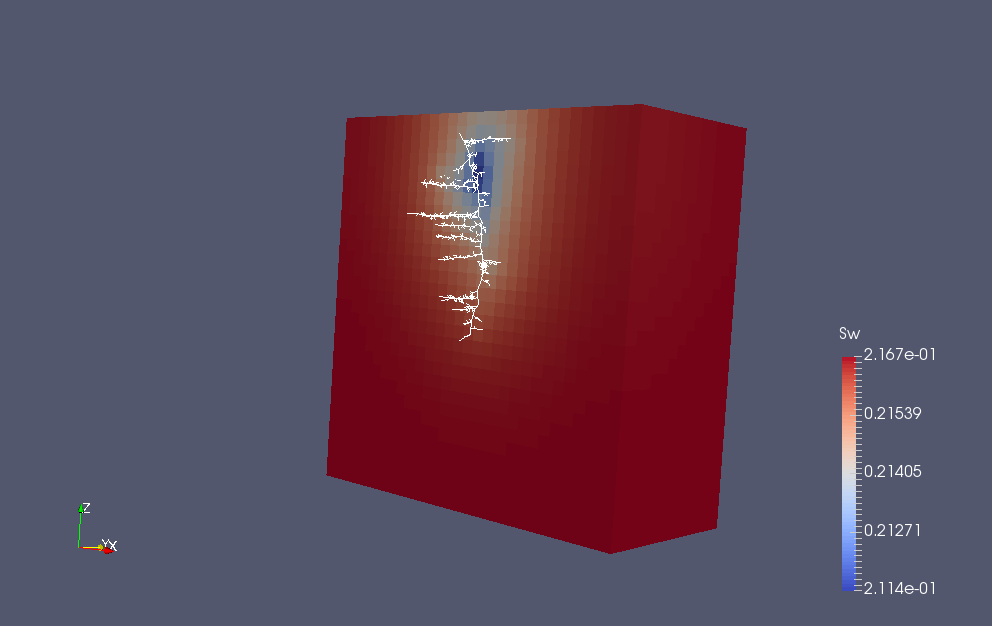
\includegraphics[width=0.8\textwidth]{RWU.png}
	\captionsetup{labelformat=empty}
	\caption{Visualisation of soil saturation as affected by root water uptake.}
	\label{RWU}
\end{figure}

\todo[inline]{output transpiration over time!}